\documentclass[conference]{IEEEtran}
\IEEEoverridecommandlockouts
% The preceding line is only needed to identify funding in the first footnote. If that is unneeded, please comment it out.
\usepackage{cite}
\usepackage{amsmath,amssymb,amsfonts}
\usepackage{algorithmic}
\usepackage{graphicx}
\usepackage{textcomp}
\usepackage{xcolor}
\usepackage{multirow}
\def\BibTeX{{\rm B\kern-.05em{\sc i\kern-.025em b}\kern-.08em
    T\kern-.1667em\lower.7ex\hbox{E}\kern-.125emX}}
\begin{document}

\title{Comparing Reinforcement Learning and Finite State Machine Agents in Real Time Strategy Games: Impact on Player Experience}

\author{\IEEEauthorblockN{Joshua Polanszky}
\IEEEauthorblockA{\textit{Institute of Information Communication Technology} \\
\textit{Malta College of Arts Science and Technology}}
Paola, Malta
}

\date{\today}

\maketitle

\begin{abstract}
abstract
\end{abstract}

\begin{IEEEkeywords}
Keywords
\end{IEEEkeywords}

\section{Introduction}

% Introduction Section. Example citations: \cite{ronneberger2015unet} and \cite{latex2e}
% TODO: Restructure a bit
\subsection{Theme and Topic Rationale}
% TODO: Cite the papers taken from the dissertation that are relevant to the topic, since the topic is similar to the disseration and as such, I already have the info i need without re reading.

The Theme chosen is Decision-Making AI for Real-Time Strategy (RTS) Games, and will focus on comparing Finite State-Machine (FSMs) AI opponents traditionally used in games, against Machine Learning (ML) opponents, specifically 
Reinforcement Learning (RL), and their impact on player experience. 

Game AI plays a huge role in player experience and immersion, as they provide the challenge and unpredictability that makes games fun and engaging.
While extensive research has been conducted on the topic, few have compared the experience these AI opponents provide to players, and focused more on the pure performance of the RL agent, rather than the
player experience. This study aims to address the research gap by directly comparing RL Agents to FSMs, and evaluating their impact on player experience, with the goal of identifying if the computational
and development cost of implementing RL agents is justified by the improvement in player experience.

\subsection{Positioning and Research Onion}

This research will be positioned within the gap of player experience found in literature, and will help in provided a better understanding on the role RL agents will play in the future of RTS games, building off of the
work done by \cite{vinyals_grandmaster_2019} in their work on AlphaStar.

As can be seen in Figure \ref{fig:research_onion}, this study will follow a positivist research paradigm, following a deductive and experimental approach, gathering both quantitative and qualitative data to measure player experience.

\begin{figure}[htbp]
    \centering
    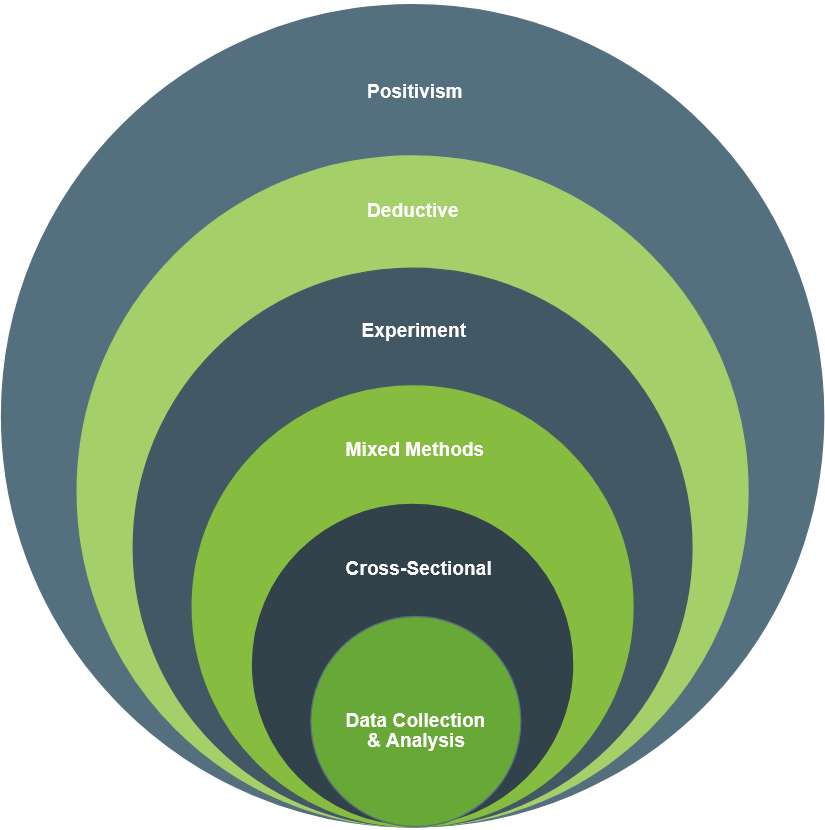
\includegraphics[width=0.45\textwidth]{../Images/Research_Onion.PNG}
    \caption{Research Onion}
    \label{fig:research_onion}
\end{figure}

\subsection{Background to the Research Theme}
% TODO: Add references to papers from dissertation, and maybe expand
Game AI has evolved significantly over the years, especially in RTS games. Early RTS titles, such as StarCraft, relied on Finite State Machines (FSMs) for their AI decision-making. These FSM-based approached
are deterministic and predictable, which can lead to repetitive and boring gameplay, and allow players to exploit the gameplay patters of the AI.

More recently, RL has emerged as an alternative AI approach, taking advantage of advancements in ML and computer hardware. In games such as AlphaStar \cite{vinyals_grandmaster_2019}, RL agents were able to 
demonstrate adaptive and human-like behaviour, providing a more challenging and engaging experience for players. Despite all of this, the implementation of RL in commercial games remains limited due to
the high computational cost, long training and development times, and added complexity. 

This further proves the need for research in this area, and in evaluating if the benefits of RL agents in RTS games are worth the cost compared to traditional FSMs.

\subsection{Hypothesis}

Players report a higher level of enjoyment and improved experience when playing against RL agents comparted to FSMs in RTS games.

\subsection{Independent \& Dependent Variables}

% Explain the difference between independent and dependent variables

In this study, there will only be 1 independent variable, and that is the type of AI opponent. As for dependant variables, there will be multiple, with those being player experience, player immersion, and 
perceived difficulty. Player experience will be measured through surveys and engagement metrics, player immersion will be measured through surveys and validated game design principles, and perceived difficulty
will be measured through surveys, player feedback, and engagement metrics.

\subsection{Research Aim}

The aim of this study is to evaluate the impact of Reinforcement Learning (RL) and Finite State Machines (FSMs) AI opponents on player experience in Real-Time Strategy (RTS) games, and determine if the extra resources
is justified by the improvement in player experience for RL agents.

To be more specific, the study will focus on the following research objectives:

\begin{itemize}
    \item Compare player-reported enjoyment and engagement levels when playing against RL and FSM AI opponents in RTS games.
    \item Assess the impact of RL and FSM AI opponents on player immersion in RTS games.
    \item Determine if the computational and development costs and complexity of RL justify its implementation over FSMs in RTS games.
\end{itemize}

\subsection{Purpose Statement}

This study is important because AI opponents shaoe the core gameplay experience of RTS games. While FSMs remain widely used due to their simplicity, RL-based AI has the potential to revolutionise
RTS games by providing adaptive and unpredictable opponents. However, the significant resource demand from developers raise questions if the benefits of RL are worth the investment.

By investigating the difference in player experience between RL and FSM AI, this study will provide valuable insights to game developers, AI designers, and the broader gaming community, helping them
in making more informed decisions regarding AI decision-making strategies in RTS game development.

\section{Literature Review}

Literature review goes here

\section{Research Methodology}

Research Methodology goes here

\section{Findings}

Findings go here

\section{Conclusion}

Conclusion goes here:

\bibliographystyle{ieeetr}
\bibliography{references}
\end{document}
